% !TEX root = ../main.tex
\section{Methodology}
\label{sec:methodology}

With the answer representation fixed, we learn a conditional generator over complete reasoning traces. Our denoising and token-decoding objectives closely follow ELF \citep{elf}. The principal changes concern the representation being generated and how the question is encoded and introduced during training (Figure~\ref{fig:pipelineoverview}).

\subsection{Flow matching and shared token decoding}
\label{sec:methodflow}

\paragraph{Continuous denoising.}
Let $x\in\R^{T\times d}$ collect the clean answer latents from Section~\ref{sec:representation}, with $d=1024$, and let $c$ denote the clean question representation. Flow matching \citep{flowmatching} learns a vector field that transports a simple noise distribution to the conditional data distribution. We use the linear interpolation
\begin{equation}
 z_t=t x+(1-t)\sigma\epsilon,
 \qquad \epsilon\sim\mathcal N(0,I),\quad \sigma=2,\quad t\in[0,1].
 \label{eq:methodinterpolant}
\end{equation}
The path starts at noise and ends at the teacher-derived answer. One time is drawn per training example and shared across its tokens and layer groups. Question positions remain clean; a bidirectional Transformer jointly processes the question and noisy answer.

Following ELF, the network $F_\theta$ predicts the clean endpoint. Its inputs include the current state, time, question condition, and an optional previous clean prediction $s$ for self-conditioning. We convert the endpoint prediction to a velocity using ELF's stabilized denominator:
\begin{equation}
 v_\theta=\frac{F_\theta(z_t,t,c,s)-z_t}{\Delta_t},
 \qquad v^*=\frac{x-z_t}{\Delta_t},
 \qquad \Delta_t=\max(1-t,0.05).
 \label{eq:methodvelocity}
\end{equation}
Away from the clamp, $v^*=x-\sigma\epsilon$ is the path velocity. For a microbatch of examples $r$ with response mask $M_{rj}$, the basic flow-matching loss is
\begin{equation}
 \mathcal L_{\mathrm{FM}}=
 \E\!\left[\frac{\sum_{rj} M_{rj}\|v_{\theta,rj}-v_{rj}^*\|_2^2}
 {d\sum_{rj} M_{rj}}\right].
 \label{eq:methodflowloss}
\end{equation}
All latent coordinates contribute to this loss; padding and question positions are excluded.

\paragraph{Self-conditioning and SCCFG.}
Self-conditioning supplies an earlier clean prediction to the denoiser, allowing successive predictions to refine one another. We inherit ELF's self-conditioning classifier-free guidance (SCCFG), which strengthens this signal by training the network to produce guided predictions. The guidance scale is an input to the model, so sampling uses one denoiser call per step. In our conditional setup, the comparison underlying SCCFG is between predictions with and without \emph{answer self-conditioning}; the question remains present in both. Training replaces $v^*$ in Eq.~\eqref{eq:methodflowloss} by a detached guidance-adjusted target $\widetilde v^*$. Appendix~\ref{app:methodobjective} gives the target and sampling distributions.

\paragraph{Recovering discrete tokens.}
A token head on the same Transformer backbone maps answer latents to vocabulary probabilities $p_\theta^{\mathrm{dec}}$. Decoder-mode training uses a separate corruption $z^{\mathrm{dec}}$ of the clean answer and same-position token labels $y_j$:
\begin{equation}
 \mathcal L_{\mathrm{CE}}=
 \E\!\left[-\frac{\sum_{rj} M_{rj}\log p_\theta^{\mathrm{dec}}(y_{rj}\mid z_r^{\mathrm{dec}},c_r)}
 {\sum_{rj} M_{rj}}\right].
 \label{eq:methoddecoderloss}
\end{equation}
Each training row selects flow mode with probability $0.8$ or decoder mode with probability $0.2$. Thus the expected mixture is $0.8\mathcal L_{\mathrm{FM}}^{\mathrm{SCCFG}}+0.2\mathcal L_{\mathrm{CE}}$, using a common valid-token normalization in each microbatch. The backbone is shared between modes, with separate continuous and vocabulary output heads. At generation time, states remain continuous throughout denoising; a final call through the backbone and token head decodes the complete answer in parallel. This training construction remains close to the original ELF formulation, with the exact masks and decoder corruption specified in Appendix~\ref{app:methodobjective}.

\subsection{Learning the conditional encoding in three stages}
\label{sec:conditionalencoding}

\paragraph{Token embedding versus contextual encoding.}
An \emph{embedding} is a token-local linear map: for a vocabulary table $B_\psi$, $e_j=B_\psi[q_j]$ depends only on token $q_j$ and is equivalent to multiplying its one-hot vector by a matrix. An \emph{encoding} is a contextual computation, $c_j=P_\phi(e_1,\ldots,e_{L_q})_j$, that combines information across the question using a Transformer. Our learned prompt encoder attends bidirectionally within the question; the original Qwen encoding instead respects the teacher's causal mask. Both supply contextual information beyond a token lookup.

ELF obtains its conditional representations from a frozen T5 encoder \citep{elf}, and REPA+REG retains a frozen Qwen3-0.6B-Base encoder for inference-time prompts \citep{scalingdlm}. This provides informative conditioning but preserves a dependency on an external contextual encoder, whose representation is fixed rather than adapted to the denoiser. We replace the teacher Transformer with a compact, trainable prompt encoder while retaining the frozen Qwen token embedding table. The student has six bidirectional Transformer blocks and outputs the same 1,024-dimensional interface as the teacher features. Once trained, it encodes the question once per response; no Qwen Transformer layers are executed at inference.

Our curriculum separates establishing the conditional generator from learning its conditioning interface:
\begin{enumerate}
 \item \textbf{Train ELF under frozen Qwen conditioning.}
 For the first 12 ELF epochs, use the projected question-only teacher states $c_{\mathrm T}(q)$ and optimize the flow/decoder objective. The teacher and representation projectors remain frozen, giving the denoiser a stable, informative condition throughout its initial training.

 \item \textbf{Fit the prompt encoder by imitation.}
 Hold ELF fixed and train $P_\phi$ to match the teacher question states:
 \begin{equation}
  \mathcal L_{\mathrm{prompt}}=
  \E_q\!\left[\frac{1}{L_qd}\sum_{j=1}^{L_q}
  \|P_\phi(q)_j-c_{\mathrm T,j}(q)\|_2^2\right].
  \label{eq:methodpromptmse}
 \end{equation}
 Here $P_\phi(q)$ includes the frozen token lookup followed by the trainable contextual encoder. Each question has equal weight, and padding is excluded. This stage learns a compatible initialization without advancing ELF's training epoch.

 \item \textbf{Adapt the prompt encoder and ELF jointly.}
 Substitute $P_\phi(q)$ for $c_{\mathrm T}(q)$ at ELF epoch 12 and resume the same flow/decoder training, updating both networks. Answer targets and the vocabulary lookup remain fixed. We apply no additional prompt-MSE objective: the encoder now adapts through the downstream generative losses. Joint training continues to epoch 18 for ELF-B and epoch 21 for ELF-L.
\end{enumerate}

% !TEX root = ../main.tex
\begin{figure}[htbp]
\centering
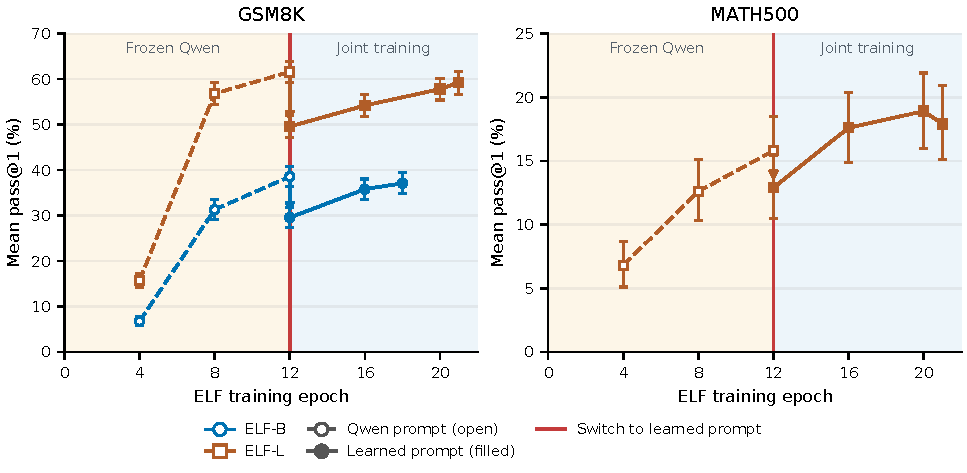
\includegraphics[width=\linewidth]{figures/prompt_curriculum_training.pdf}
\caption{\textbf{Stable teacher conditioning followed by learned prompt adaptation.} Pre-NFT learning curves, with GSM8K ELF-B/L together on the left and MATH500 ELF-L on the right. Open circles use Qwen prompt encoding; filled squares use the learned encoder. The vertical bar marks the epoch-12 substitution and start of joint training; arrows show the immediate MSE-prompt swap loss. Standalone prompt-MSE training leaves the ELF epoch fixed. Both axes start at zero; the first evaluated checkpoint is epoch 4. Points average seeds 42/123 at async $(2.5,2,1.5)$, 32 steps, and SCCFG 2; bars are 95\% problem-bootstrap intervals. ELF EMA is $0.9999$; prompt EMA is $0.999$ at the swap and $0.9999$ afterward.}
\label{fig:promptcurriculum}
\end{figure}


Figure~\ref{fig:promptcurriculum} shows why imitation and downstream adaptation serve different roles. The MSE-trained encoder causes an immediate accuracy drop, even though the ELF checkpoint is unchanged at the swap. Joint training then recovers much of this loss on GSM8K and surpasses the original epoch-12 teacher-conditioned accuracy on MATH500. For example, the MATH500 curve moves from 15.80\% with Qwen conditioning to 12.90\% after substitution and 17.90\% after joint training. Recovery reflects adaptation of \emph{both} ELF and its prompt encoder. Matching latent coordinates provides a useful starting point, while the generative objective determines how the condition should ultimately be used.

\subsection{Why keep the conditioning fixed initially?}
\label{sec:conditioningcurriculum}

Learning the conditioning representation and the conditional flow simultaneously couples two difficult problems: the denoiser must learn to interpret a representation that is itself changing, while the encoder receives supervision through an immature denoiser. We therefore use the teacher encoding as a fixed target during the period in which the flow model learns its initial conditional structure, and allow task-specific adaptation only after that structure has formed.

The joint-from-start control in Figure~\ref{fig:representationcomparison} supports this curriculum. With the same learned answer representation, a randomly initialized prompt encoder trained alongside ELF reaches only \textbf{8.70\%} GSM8K accuracy at epoch six, compared with \textbf{30.76\%} under frozen teacher conditioning. The contrast shows the importance of anchoring early learning in an informative, stable condition within the tested training budget. The subsequent joint-training curves show that the value of this anchor is compatible with later adaptation.

This perspective connects to REPA \citep{repa}, where external pretrained features ease the representation-learning burden of a diffusion model and accelerate training. Here the teacher supplies structure through the \emph{conditioning interface}. We interpret the comparison as evidence for a related curriculum principle: establish the conditional generative model under stable teacher guidance before asking it to reshape that guidance. The precise contribution of feature drift versus the initial quality of the prompt representation remains an open mechanism; the practical implication is that \emph{when conditioning becomes learnable} is an important design choice alongside its architecture.

% Asynchronous denoising and its mathematical formulation will be drafted after
% the user's next discussion; no inference subsection is added in this revision.
